\documentclass[hyperref={pdfpagelabels=false}]{beamer}
\usepackage{beamerthemesplit}
\usepackage[utf8]{inputenc}
\usepackage[T1]{fontenc}
\usepackage{lmodern}
\usepackage{graphicx}

\usetheme{Green}

\begin{document}
  \title{CoqOfOCaml}
  \author{Guillaume Claret}
  \date{5 September 2014}
  \maketitle

  \section{Introduction}
  \begin{frame}
    \frametitle{Two languages}
    \emph{OCaml}:
    \begin{itemize}
      \item programming language
      \item functional programming with imperative features
      \item many libraries and programs
    \end{itemize}
    \emph{Coq}:
    \begin{itemize}
      \item (mainly used as a) proof language
      \item purely functional programming (not even non-termination)
      \item dependent types
      \item limited number of libraries for the programmer
    \end{itemize}
  \end{frame}
  \begin{frame}
    \frametitle{Bridges}
    \emph{Coq} to \emph{OCaml}: extraction mechanism:
    \begin{itemize}
      \item developed mainly by Pierre Letouzey
      \item removes the proof terms
      \item converts the remaining purely functional expressions to \emph{OCaml}
      \item complete
    \end{itemize}
    \emph{OCaml} to \emph{Coq}:
    \begin{itemize}
      \item \emph{CFML}: deep embedding
      \item how to do shallow embedding?
      \item how to import imperative programs?
    \end{itemize}
  \end{frame}
  \begin{frame}
    \frametitle{CopOfOCaml}
    \begin{center}
      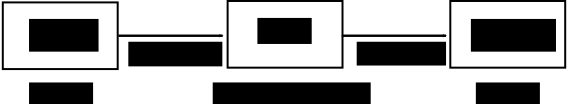
\includegraphics[width=10cm]{images/compilation_chain}
    \end{center}
    We use a \emph{monadic translation} to represent imperative features in~\emph{Coq}.
  \end{frame}
  \begin{frame}
    \frametitle{Usages}
    You may want to:
    \begin{itemize}
      \item prove formal properties on \emph{OCaml} programs
      \item augment the number of \emph{Coq} libraries for programming
    \end{itemize}
  \end{frame}
  \begin{frame}
    \frametitle{Informal specification}
    The following programs are equivalent (same input-output traces):
    \begin{itemize}
      \item \texttt{foo.ml} and \texttt{foo.v} (interpreting the monad)
      \item \texttt{foo.v} and \texttt{foo2.ml}
    \end{itemize}
    Not proved.
  \end{frame}
  \begin{frame}
    \frametitle{Quick demo}
    {\Huge Quick demo.}
  \end{frame}

  \section{Effects system}
  \begin{frame}
    \frametitle{Effects system}
    \begin{center}
      
\includegraphics[width=4cm]{images/effects}
    \end{center}
    \begin{center}
      How imperative features (\emph{effects}) are inferred and represented in~\emph{Coq}.
    \end{center}
  \end{frame}
  \begin{frame}
    \frametitle{Effects}
    For now simple effects:
    \begin{itemize}
      \item no polymorphism
      \item no function arguments with effects
    \end{itemize}
    \begin{block}{Effects descriptor}
      A set of atomic effects (exceptions, top-level references, input-output):
      \[
        d := \{ a_1, \dots, a_n \}
      \]
    \end{block}
  \end{frame}
  \begin{frame}
    \frametitle{Effects}
    \begin{block}{Effect type}
      The shape of an \emph{OCaml} type with effects:
      \[
        \begin{array}{rcl}
          \tau &:=& \mathrm{Pure}\\
               &|& \mathrm{Pure} \xrightarrow{d} \tau
        \end{array}
      \]
    \end{block}
    \begin{block}{Effect of an expression}
      \begin{itemize}
        \item the effect type
        \item a descriptor of the effects used to evaluate it
      \end{itemize}
    \end{block}
  \end{frame}
  \begin{frame}
    \frametitle{Example}
    For the expression:

    \texttt{print\_endline "will fail";\\(fun x -> failwith "error")}

    we have the effect:
    \[
      (\mathrm{Pure} \xrightarrow{\{\mathtt{OCaml.Failure}\}} \mathrm{Pure}, \{\mathtt{IO}\})
    \]
  \end{frame}
  \begin{frame}
    \frametitle{Inference of effects}
    \begin{itemize}
      \item first: inference of types using the \emph{OCaml} compiler
      \item then: bottom-up analysis
      \item fixpoint for mutually-recursive definitions
    \end{itemize}
  \end{frame}
  \begin{frame}
    \frametitle{Effects in \emph{Coq}}
    Using monads:
    \begin{center}
      $M\,A$: type of computations in the monad $M$ returning a value of type $A$
    \end{center}
    Operators:
    \[
      \begin{array}{l}
      \mathrm{return} : \forall A, A \rightarrow M\,A\\
      \mathrm{bind} : \forall A\,B, M\,A \rightarrow (A \rightarrow M\,B) \rightarrow M\,B
      \end{array}
    \]
  \end{frame}
  \begin{frame}
    \frametitle{Composition of monads}
    There is one monad per descriptor of effects $d$. How to compose them?

    The monadic composition is not possible in general. Solution: we constrain the shape of the monads:
    \[
      M_d\,A = (S_1 \times \cdots \times S_n) \rightarrow (A + E_1 + \cdots + E_n) \times (S_1 \times \cdots \times S_n)
    \]
    with: $S_i$ states, $E_i$ exceptions.
  \end{frame}
  \begin{frame}
    \frametitle{Composition of monads}
    Commutative composition of $M_{d_1}$ and $M_{d_2}$:
    \[
      M_{d_1 \cup d_2}
    \]
    Lift operator:
    \[
      \mathrm{lift}_{d, d'} : \forall A, M_d\,A \rightarrow M_{d'}\,A
    \]
    (if $d \subseteq d'$).
  \end{frame}
  \begin{frame}
    \frametitle{List of effects}
    \begin{itemize}
      \item references
      \item exceptions
      \item inputs/outputs (a reference to an abstract world)
      \item non-termination: using a fuel
    \end{itemize}
  \end{frame}

  \section{Implementation}
  \begin{frame}
    \frametitle{Implementation}
    \begin{center}
      
\includegraphics[width=4cm]{images/implementation}
    \end{center}
  \end{frame}

  \section{Case studies}

  \section{Conclusion}
\end{document}